This section present all details about RoboFEI@Home software. A stable version of the software is available on GitHub\footnote{https://github.com/OpenFEI/rfh\_judite}. Follow sections are divided as: (I) Software Architecture of Judith; (II) Face and People Recognition; (III) Object Detection; (IV) Speech Recognition and Synthesize; (V) Navigation; (VI) Object Manipulation.

\subsection{Software Architecture}\label{architecture}
All Judith software is developed using Ubuntu Linux 14.04 LTS~\cite{sobell:2014} and ROS Indigo Igloo~\cite{ros:2015}. The initial architecture of Judith is composed by three layers. Each layer is responsible for one part of the code. First layer receives all data from sensors, extract the features and publish it for AI and Controller nodes (Second Layer). AI and Controller nodes take the features and run algorithms for computer vision, location, planning, pattern recognition, among others. In the end, second layer send to third layer what is the velocity of the motors, position of manipulator or face express by robot. Third layer controls all the actuators drivers and actions. A graphic view of the architecture is presented on Fig.~\ref{fig:architecture}.

\begin{figure}[ht!]
    \centering
    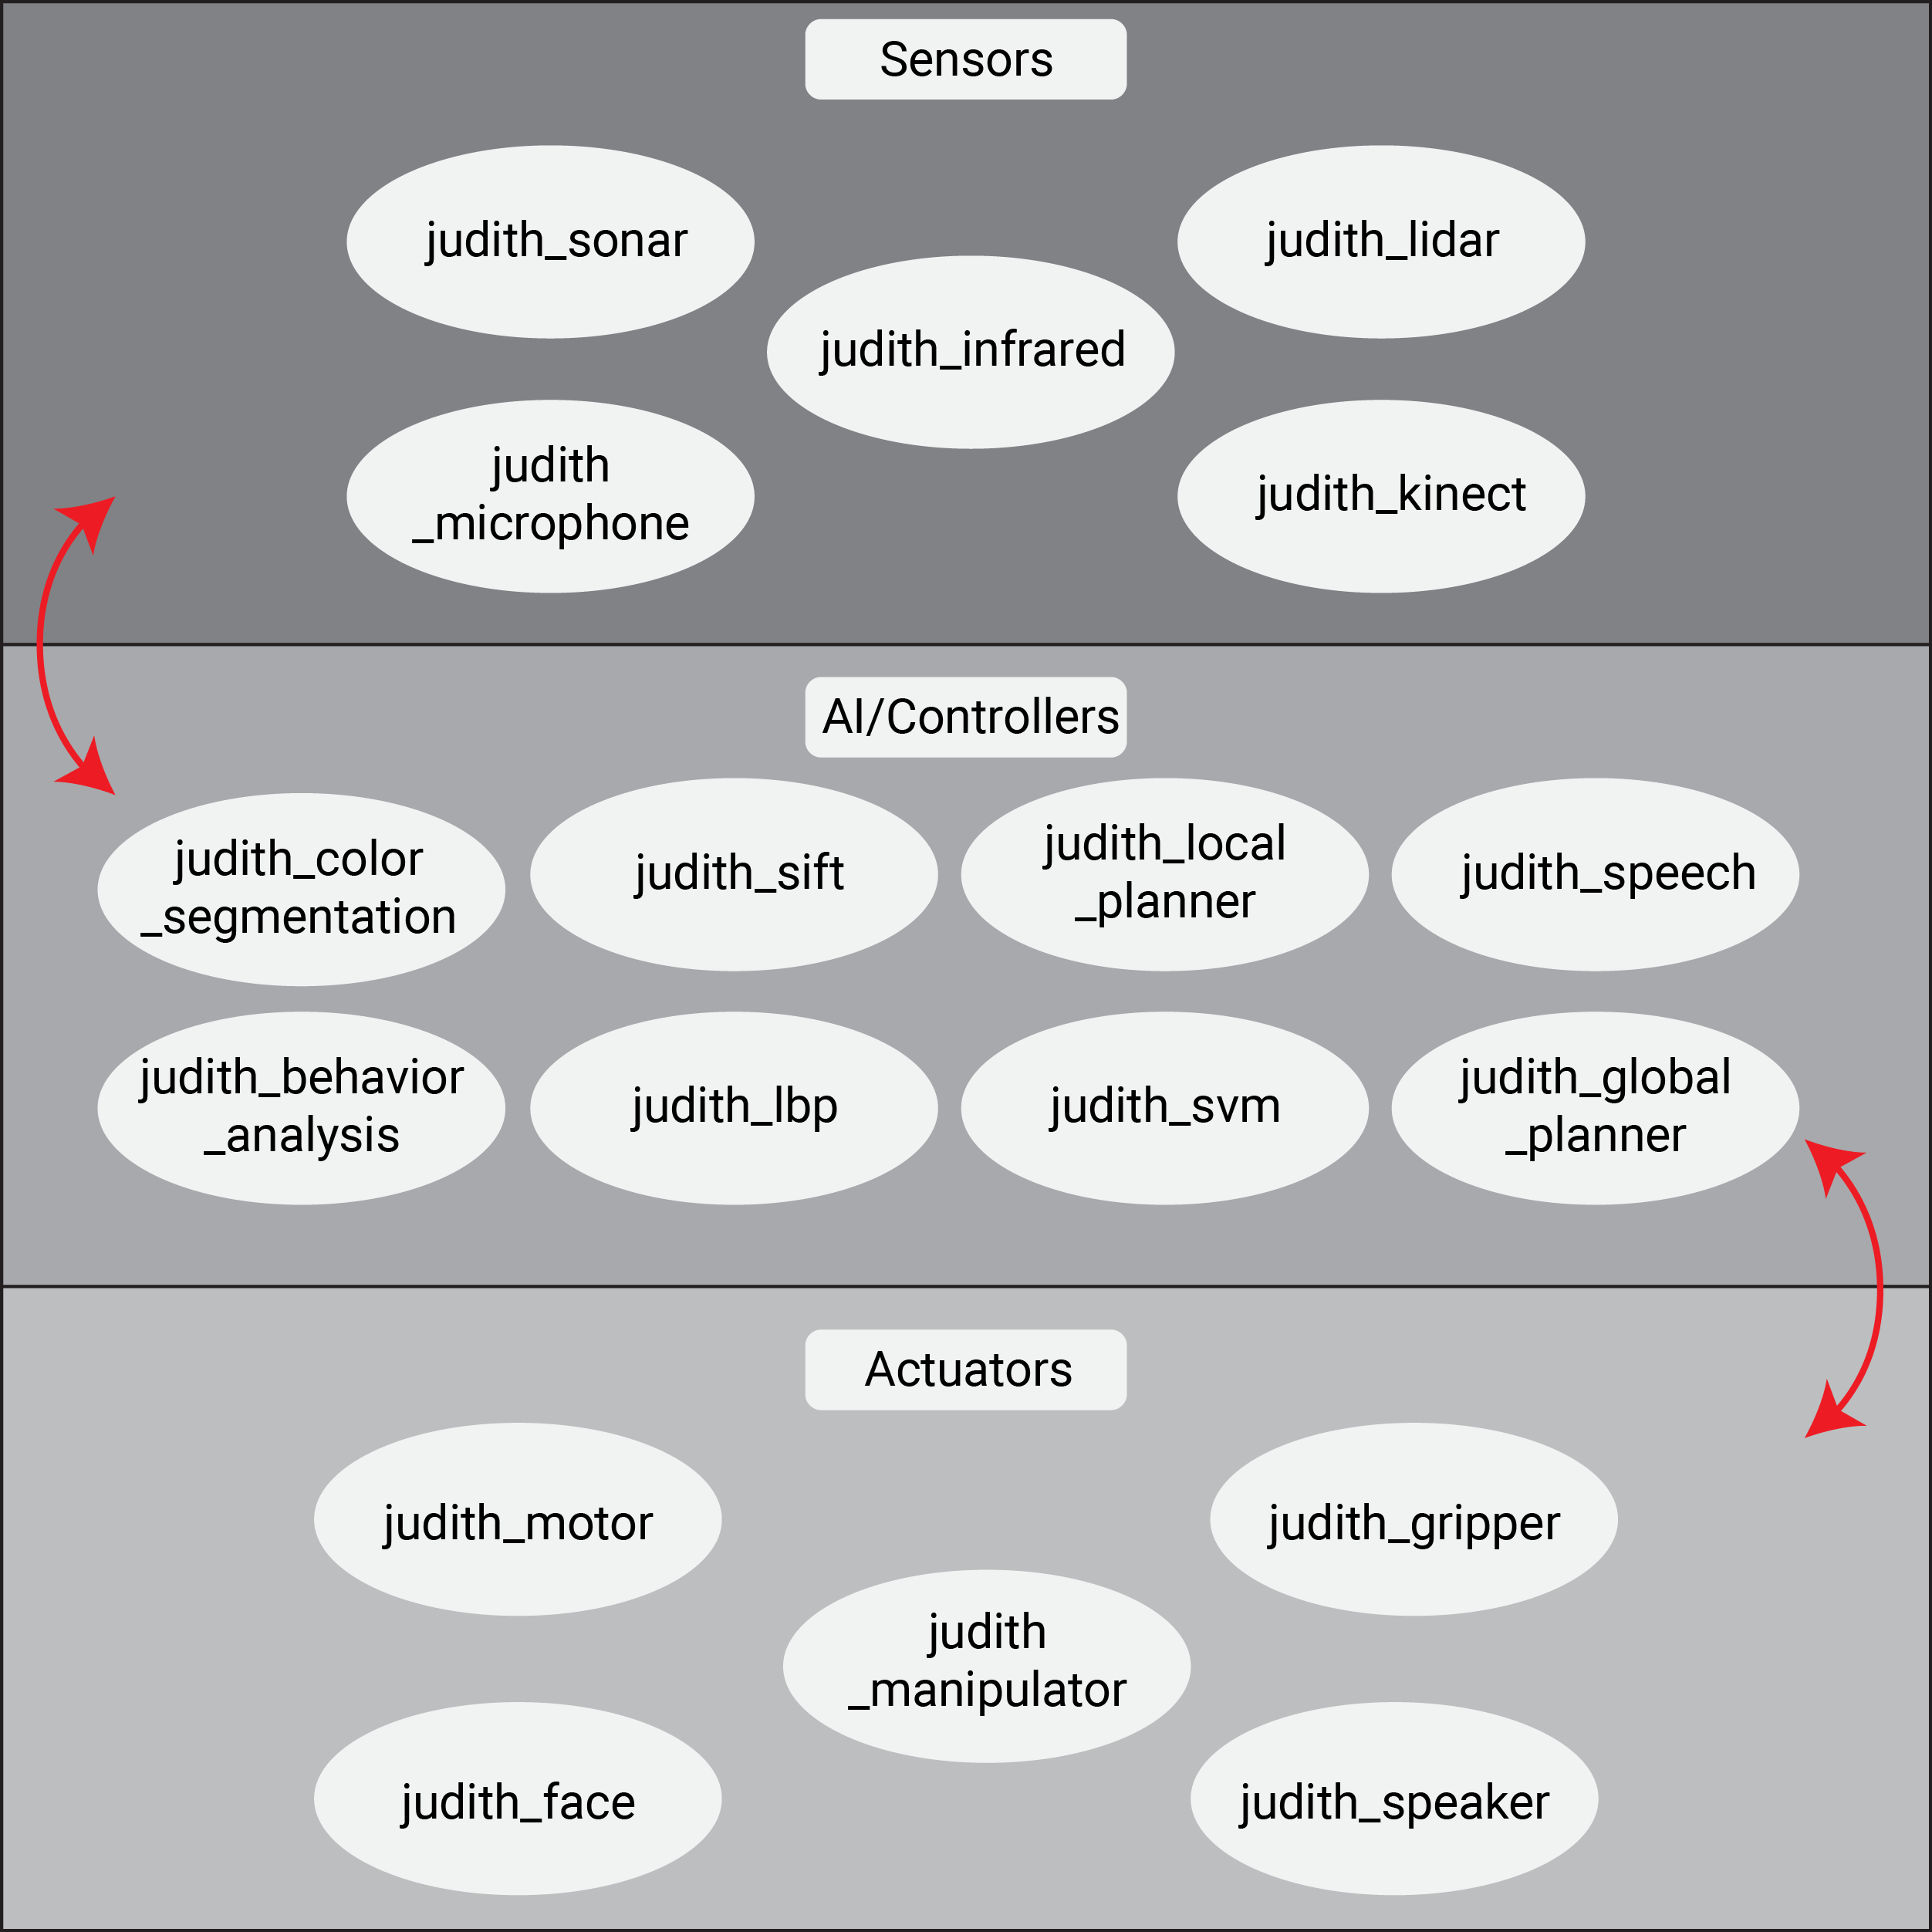
\includegraphics[width = \textwidth]{figures/architecture.png}
    \caption{Software Architecture of Judith}
    \label{fig:architecture}
\end{figure}

Sensors and Actuators layers has been developed using C++~\cite{stroustrup:1986}, due to hardware drivers communication, except by judith\_face node. Face's node is developed in Java~\cite{joy:2000} language to create an application on Android~\cite{android:2016} Platform. AI/Controllers layer is developed using Python~\cite{vanrossum:2010} as programming language to all algorithms. All decisions made for the best performance of our robot during task execution and also for training new members to the team.

\subsection{Face and People Recognition}\label{face-people-recognition}
We understand when you recognize a person and treat it by the name, you make the interaction more comfortable for her/him. In that way, we develop some nodes that can detect and recognize a person by their face. To make it possible, we acquire an image using a camera (Webcam Logitech C920 or Microsoft Kinect X360) and convert the frame into a OpenCV~\cite{bradski:2000} Image Matrix. This information is a input of the LBP algorithm which has been widely used for face recognition due to its computational performance~\cite{ahonen:2006,yang:2007,shan:2012,ylioinas:2012,samadi:2013}. LBP algorithm may also help on identify gender, age and facial expression which can be useful for making an adaptive behavior of the robot during interaction.

Beyond facial recognition this set of nodes is responsible for following a single person, without external interference during process. To perform this task, we decide to combine three techniques. First is face detection followed by extraction of the color from person t-shirt~\cite{pulli:2012,laganiere:2011,baggio:2012}. With the t-shirt color defined, we perform a color segmentation using OpenCV~\cite{kang:2008,oliveira:2009,culjak:2012}. The last technique is to extract a skeleton position using Nite/OpenNI library for Microsoft Kinect~\cite{openni:2011}. With this information robot can follow the direction of a certain person and also to identify the distance between them.

\subsection{Object Detection}\label{object-detection}

\subsection{Speech Recognition and Synthesize}\label{speech}
Speech is one of the most important way to interact with a human. Due to that, we use CMU Pocketsphinx~\cite{huggins:2006} to make Judith's speech recognition and also synthesize a female voice on our robot.

\subsection{Navigation Stack}\label{navigation}
To execute tasks on environment the robot needs to know where it is and how to arrive into another point of the place. The first step is create an environment map. For performing this task, we use GMapping and SLAM to create the map with laser Hokuyo URG-04LX-UG01 helps. We save the map bag using a node from ROS called map\_server.

After that, we run the bag saved and execute the algorithm \emph{Adaptive Monte Carlo Localization} (AMCL)~\cite{fox:1999} with data from the laser make the robot capable to locate its position on the map. With position known, we can give the robot a point to go on the map. Next step is to use an algorithm A* to make the route between current position and desire position. After that, for each movement of the robot, it executes an \emph{Dynamic Window Approach}(DWA) algorithm for planning the current position movements.

\subsection{Object Manipulation}\label{manipulation}
For manipulating an object, we first use object detection node (see sec.~\ref{object-detection}) to know its current position. Then we execute a few movements preview determined to put the gripper on robot view. After that, we use PCL algorithm~\cite{aldoma:2012} to segment the gripper and get object distance. At the end we execute planning to move KUKA youBot arm joints for getting closer and grab the object.
